\documentclass[a4paper,12pt]{report}

\usepackage{alltt, fancyvrb, url}
\usepackage{graphicx}
\usepackage[utf8]{inputenc}
\usepackage{hyperref}
\newcommand{\mail}[1]{\href{mailto:#1}{\texttt{#1}}}


\usepackage[italian]{babel}

\usepackage[italian]{cleveref}

\title{Relazione ``GSS'' \\ Gestionale Società Sportiva}

\author{Brini Tommaso (\mail{tommaso.brini@studio.unibo.it}) \\ Matricola 0000933814 \\ Mazzanti Gustavo (\mail{gustavo.mazzanti@studio.unibo.it}) \\ Matricola 0000914975 \\ Rambaldi Riccardo (\mail{riccardo.rambaldi4@studio.unibo.it}) \\ Matricola 0000875146}


\begin{document}

\maketitle

\tableofcontents

\chapter{Analisi dei requisiti}

Si vuole sviluppare un database a supporto della gestione di una società sportiva. La base di dati dovrà immagazzinare informazioni relative alla società in questione, ai tesserati e agli impegni in programma (allenamenti, partite, eventi vari). Il responsabile della società potrà quindi visualizzare tutti i giocatori, tutti i membri dello staff e tutti i dirigenti. Inoltre, potrà inserire nuovi eventi che verrano visualizzati in un calendario settimanale.

\section{Intervista}
Si vuole creare un gestionale per una società di calcio, di basket o di pallavolo. \newline
Si vuole innanzitutto tenere traccia delle informazioni della società, quali nome, sport, partita Iva, logo e colori sociali. \newline
Si vuole inoltre tenere traccia di tutti i tesserati della società sportiva, memorizzandone nome, cognome, codice fiscale, data di nascita, numero di matricola del tesserino, sesso, ruolo e eventualmente una foto di riconoscimento. \newline
Alla società appartengono diverse tipologie di persone: i giocatori, i membri dello staff e i dirigenti. I componenti delle prime due categorie devono appartenere a una categoria specifica (in altri termini, a una squadra). I dirigenti invece non appartengono a nessuna squadra. Ogni giocatore e ogni membro dello staff devono appartenere a una e una sola squadra, una singola persona perciò non può essere visualizzata in due categorie diverse. In aggiunta, per i giocatori è necessario salvare anche peso, altezza, la data di scadenza del certificato medico e la mano/piede preferito (a seconda dello sport selezionato). \newline
Per ogni persona ci deve essere la possibilità di salvare dei documenti visualizzabili nella scheda della persona stessa. \newline
Si vuole infine visualizzare in un calendario tutti gli impegni della società. Gli impegni possono essere di tre tipi: partite, allenamenti o eventi generici (a cui verrà assegnata una breve descrizione). A ogni partita e a ogni allenamento può partecipare solo una squadra, mentre per gli eventi generici è necessario creare una lista di convocati.


\section{Estrazione dei concetti principali}
A seguito della lettura e comprensione dei requisiti richiesti dal cliente, si procede sviluppando un testo che ne riassuma tutti i concetti principali. 
Si tiene conto delle seguenti correzioni di ambiguità.

\begin{figure}[htp]
    \centering
    \includegraphics[width = \textwidth]{GSS_report/img/ambiguità.png}
    \caption{Rilevamento delle ambiguità e correzioni proposte}
    \label{fig:umlAnalisys}
\end{figure}

L'applicazione vuole gestire una sola \textbf{Società} sportiva, scegliendo lo \textbf{Sport} tra calcio, basket o pallavolo. \newline
Innanzitutto, bisogna salvare le informazioni della società, quali nome, sport, partita Iva, colori sociali e un'\textbf{Immagine} associata. \newline
Alla società appartengono tre tipi di \textbf{Persone}: \textbf{Giocatore}, \textbf{Staff} e \textbf{Dirigente}. Per ogni persona va salvato nome, cognome, codice fiscale, data di nascita, numero di matricola del tesserino, sesso, ruolo e eventualmente un'immagine associata. \newline
I giocatori e lo staff appartengono a una specifica \textbf{Categoria}, mentre i dirigenti non appartengono a nessuna categoria. La società può avere infinite categorie.
Ogni persona può appartenere a una e una sola categoria. \newline
Per i giocatori è necessario salvare anche peso, altezza, la data di scadenza del certificato medico e la preferenza. \newline
Per ogni persona si può caricare nel database delle immagini relative ai vari documenti personali.
\newline
Si vuole infine tenere un calendario degli \textbf{Eventi}. Gli eventi da tenere in considerazione sono \textbf{Partita}, \textbf{Allenamento} ed \textbf{Evento Generico}. A quest'ultimo verrà assegnato un nome o una breve descrizione. \newline
A ogni allenamento e a ogni partita può partecipare una sola categoria. Per gli eventi generici è necessario creare una lista di convocati, scelti tra tutte le persone tesserate alla società.

\section{Elenco delle azioni principali}
\begin{itemize}
    \item Creazione di una nuova società con realtivo logo, nome, colori sociali, partita Iva e lo sport di riferimento,
    \item Creazione di una nuova categoria,
    \item Creazione di una nuova persona (Giocatore, Dirigente o Staff),
    \item Creazione di un nuovo evento con le relative convocazioni (Allenamento, Partita o Evento Generico),
    \item Visualizzazione di tutte le categorie,
    \item Visualizzazione di una singola categoria (elenco Giocatori e Staff) oppure la categoria Dirigenti,
    \item Visualizzazione scheda singola persona,
    \item Inserimento e visualizzazione documenti della persona,
    \item Modifica del risultato negli eventi di tipo Partita,
    \item Visualizzazione del calendario settimanale,
    \item Visualizzazione singolo evento,
    \item Visualizzazione convocati all'evento,
    \item Eliminazione della singola persona, con conseguente eliminazione dei documenti e delle convocazioni relative,
    \item Eliminazione del singolo evento, con conseguente eliminazione delle convocazioni relative.
\end{itemize}


\chapter{Progettazione concettuale}
\section{Schema Scheletro}
\subsection{Società}
\subsubsection{Progettazione dello schema E/R}
Lo schema scheletro della società comprende la principali entità in diretta relazione con essa.
\newline
\begin{figure}[htp]
    \centering
    \includegraphics[width = \textwidth]{GSS_report/img/società.png}
    \caption{Schema scheletro della Società}
    \label{fig:umlAnalisys}
\end{figure}
\subsubsection{Raffinamenti proposti}
L'entità \textbf{Società} deve avere una partita IVA che la identifica in modo univoco nel caso in cui, in un'ottica futura di aggiornamento, si volessero aggiungere più società al database. Inoltre, la \textbf{Società} deve avere un nome (non necessariamente univoco), due \textbf{colori sociali} (che l'utente potrà scegliere al primo avvio del programma) e infine uno stemma, rappresentato come \textbf{Immagine} in relazione 1-N \textbf{Rappresenta} con \textbf{Società}. \newline \newline
Per quanto riguardo lo \textbf{Sport}, vista la necessità di popolare le tabelle dei ruoli dei giocatori a seconda dello sport scelto, abbiamo creato una relazione 1-N \textbf{Pratica} tra \textbf{Società} e \textbf{Sport}.
\begin{figure}[htp]
    \centering
    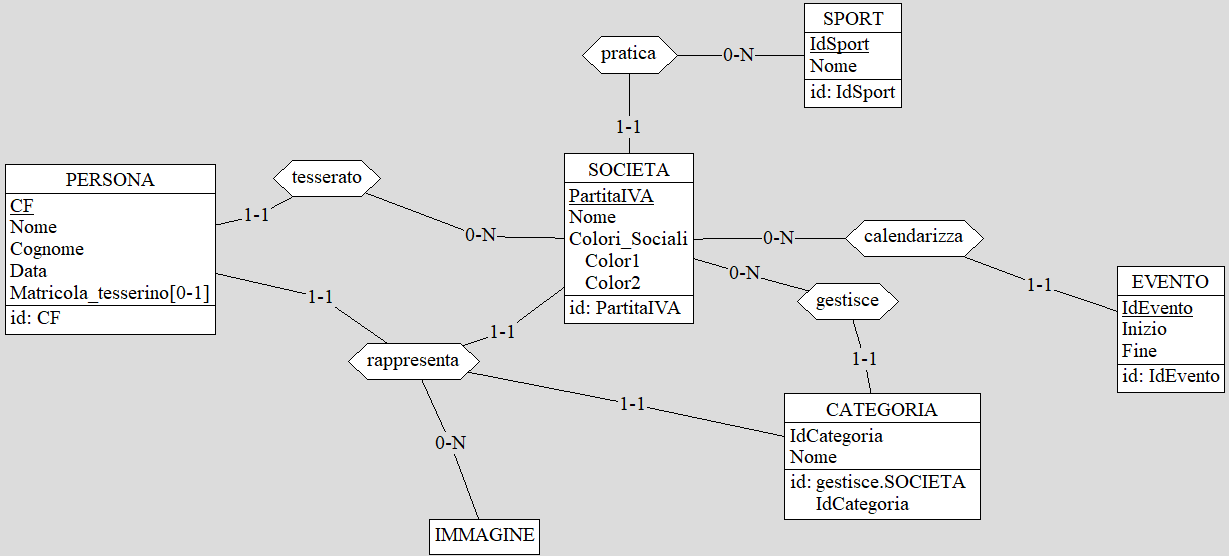
\includegraphics[width = \textwidth]{GSS_report/img/societa_raffinamento.png}
    \caption{Schema E/R parziale della Società}
    \label{fig:umlAnalisys}
\end{figure}

\newpage
\subsection{Persona}
\subsubsection{Progettazione dello schema E/R}
\begin{figure}[htp]
    \centering
    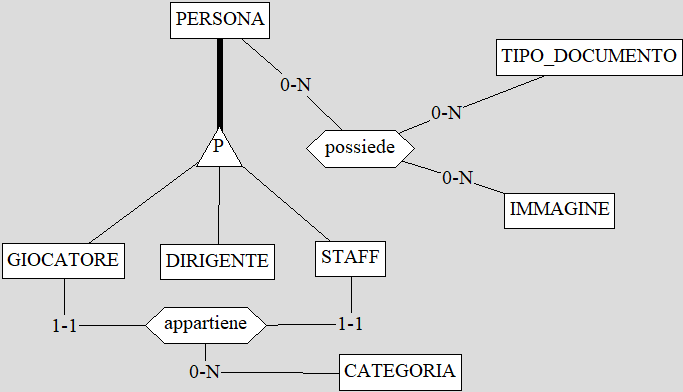
\includegraphics[width = \textwidth]{GSS_report/img/persona.png}
    \caption{Schema scheletro della Persona}
    \label{fig:umlAnalisys}
\end{figure}
\subsubsection{Raffinamenti proposti}
\section{Schema Finale}

\chapter{Progettazione logica}
\section{Stima del volume dei dati}
\section{Descrizione delle operazioni principali}
\section{Tabelle degli accessi}
\section{Raffinamento dello schema}
\section{Analisi delle ridondanze}
\section{Schema relazionale finale}
\section{Traduzione delle operazioni in query SQL}

\chapter{Progettazione dell'applicazione}
\section{Descrizione dell'architettura}

\bibliographystyle{alpha}
\bibliography{13-template}

\end{document}
